\documentclass[xcolor, handout]{beamer}

\usepackage[T1]{fontenc}

\usetheme{Malmoe}
\useoutertheme{infolines}
\useinnertheme{circles}

\makeatletter
\setbeamertemplate{mini frames}{}
\setbeamertemplate{headline}{%
	\begin{beamercolorbox}[ht=2.5ex,dp=1.125ex]{section in head/foot}
		\insertnavigation{\paperwidth}
	\end{beamercolorbox}%
}%
\makeatother
\setbeamertemplate{caption}[numbered]

% Colours defined here
\definecolor{DarkGreen}{HTML}{41964b}
\definecolor{LightGreen}{HTML}{46c755}
\definecolor{FG}{HTML}{ebebeb}
\definecolor{BG2}{HTML}{233628}
\definecolor{BG}{HTML}{202622}

\setbeamercolor{palette primary}{bg=BG, fg=FG}
\setbeamercolor{palette secondary}{bg=BG, fg=FG}
\setbeamercolor{palette tertiary}{bg=BG, fg=FG}
\setbeamercolor{palette quaternary}{bg=BG, fg=FG}

\setbeamercolor{section in head/foot}{bg=BG2, fg=DarkGreen}
\setbeamercolor{subsection in head/foot}{bg=BG2, fg=LightGreen}
\setbeamercolor{page number in head/foot}{bg=BG2, fg=LightGreen}
\setbeamercolor{author in head/foot}{bg=BG2, fg=DarkGreen}
\setbeamercolor{date in head/foot}{bg=BG2, fg=DarkGreen}
\setbeamercolor{title in head/foot}{bg=BG2, fg=LightGreen}

\setbeamercolor{normal text}{fg=FG, bg=BG}
\setbeamercolor{structure}{fg=LightGreen, bg=BG}

\setbeamerfont{subsection in toc}{size=\scriptsize}
\setbeamerfont{section in toc}{size=\footnotesize}

\usefonttheme{serif}

\usepackage{unicode-math}
\setmainfont{Gentium Basic} % Main font
\setmonofont{Fantasque Sans Mono} % Code font

\usepackage{amsmath}
\usepackage{amssymb}
\usepackage{microtype}

\usepackage{listings}
\lstset{%
	language=C,
	frame=single,
	backgroundcolor=\color{BG2},
	basicstyle={\tiny\ttfamily\color{FG}},
	keywordstyle=\color{LightGreen}
}

\usepackage{graphicx}
\graphicspath{{./files/}}

\usepackage{tikz}
\usetikzlibrary{shapes.geometric, positioning}
% tikz style
\tikzstyle{startstop} = [rectangle, rounded corners, minimum width=2cm, minimum height=1cm,text centered, draw=white]
\tikzstyle{io} = [trapezium, trapezium left angle=70, trapezium right angle=110, minimum width=2cm, minimum height=0.75cm, text centered, draw=white]
\tikzstyle{process} = [rectangle, minimum width=2cm, minimum height=1cm, text centered, draw=white]
\tikzstyle{decision} = [diamond, minimum width=2cm, minimum height=1cm, text centered, draw=white]

\usepackage{cancel}

\author[Kyu-Sang Kim]{Kyu-Sang Kim\\z5208931\\\vspace{0.2cm}Supervised by Andrew Taylor (UNSW)\\Assessed by John Shepherd (UNSW)}
\title[Thesis C Seminar]{A Testing Tool for Introductory Programming Courses}
\subtitle{Thesis C Seminar}
\date{Term 3, 2022}

\begin{document}

\begin{frame}
	\titlepage
\end{frame}

\AtBeginSection[]{
	\begin{frame}
		\frametitle{Contents}

		\centering
		\begin{columns}
			\begin{column}{0.75\textwidth}
				\tableofcontents[currentsection]
			\end{column}
			\begin{column}{0.15\textwidth}
				% Use this for anything you want to display alongside the contents
			\end{column}
		\end{columns}
	\end{frame}
}

\section{Introduction}
\subsection{Autotest - Andrew Taylor}
\begin{frame}
	\frametitle{Autotest - Introduction}
	\begin{itemize}
		\setlength\itemsep{1em}
		\item Autotest is a general code testing tool developed by Andrew Taylor
			\pause
		\item First introduced to UNSW in COMP2041 2015 S2
			\pause
		\item Currently used to perform automated marking for most UNSW introductory programming courses which has become mandatory to reduce staff workload with increasing enrolment numbers
			\begin{itemize}
				\item \textbf{COMP1521:} 715 (2017) $\rightarrow$ 1633 (2021)
			\end{itemize}
			\pause
		\item Written in Python (+ some Shell and Perl script interfaces)
			\pause
		\item Has been in use for many sessions with different courses which has led to an abundance of example test cases for a multitude of assignment types
	\end{itemize}
\end{frame}
\begin{frame}
	\frametitle{Autotest - Issues}
	\begin{itemize}
		\setlength\itemsep{1em}
		\item Has some \textbf{design deficiencies} and accumulated non-trivial \textbf{technical debt} since introduction:
		\begin{itemize}
			\setlength\itemsep{0.5em}
			\item Single-thread design does not utilise all potential processing power that is available to autotest
				\pause
			\item Vulnerable to unintended or malicious actions when autotesting user-provided programs
				\pause
			\item Design is highly coupled with low cohesion making improvements significantly more difficult to implement
				\pause
			\item Documentation in regard to crucial autotest components were lacking or non-existent which made it difficult to understand
				\pause
		\end{itemize}
		\item A refactoring or re-write of the autotest package would provide great benefit to the education of UNSW CSE students
	\end{itemize}
\end{frame}
\subsection{Thesis Statement}
\begin{frame}
	\frametitle{Thesis Statement}
	\textbf{A user-friendly and maintainable general code testing tool is important to streamline the administration of introductory programming courses}
	\\~\\
	\pause
	We will:
	\pause
	\begin{enumerate}
		\item Develop an extensible and easy to use software package which parses and runs pre-written tests on submitted code
		\pause
		\item Implement development procedures that minimise both current and future technical debt
		\pause
		\item Remediate known flaws in the existing autotest package
		\pause
		\item Maintain backwards compatibility with legacy tests written for the existing autotest package
		\pause
		\item Perform proving and performance tests on the new software package
	\end{enumerate}
\end{frame}

\section{Design}
\subsection{Design Considerations}
\begin{frame}
	\frametitle{Design Considerations}
	The design requirements of the solution emphasised the following properties in accordance with the thesis goals:\\
	\begin{itemize}
		\setlength\itemsep{1em}
		\item \textit{Accessible} - Users of the new software package should have the easiest possible experience in integrating automatic testing and grading into their courses
			\pause
		\item \textit{Familiar} - Users who have previously utilised Andrew Taylor autotest should not feel the new software package to be completely independent of the former
			\pause
		\item \textit{Performant/Efficient} - The new software package should have the same, if not better performance than the original Andrew Taylor autotest overall
	\end{itemize}
\end{frame}
\begin{frame}
	\frametitle{Design Considerations - continued}
	\begin{itemize}
		\setlength\itemsep{1em}
		\item \textit{Maintainable} - The new software package should be adequately documented and support ease of maintainability and possible extension of features via the appropriate architectural decisions
			\pause
		\item \textit{Secure} - The new software package should provide reasonable security measures to ensure that any damage by the package on the host system is minimised as much as possible
	\end{itemize}
\end{frame}
\begin{frame}
	\frametitle{Exclusions}
	\begin{itemize}
		\setlength\itemsep{1em}
		\item \textit{Novelty} - We assume novelty to be out of scope as introducing a novel user experience is in conflict with the aforementioned design requirements
			\pause
		\item Users of the existing Andrew Taylor autotest may elect to not utilise the new software package if the transition requires significant work
	\end{itemize}
\end{frame}
\subsection{Modular Design}
\begin{frame}
	\frametitle{Modular Design}
	\begin{itemize}
		\item A modular design has been selected for the new autotest
			\pause
		\item Modules are an established design pattern that fits the purpose of autotest
			\pause
		\item Enables easier swapping of components with minimal to no code changes other than import statements
			\pause
		\item Maintenance and Improvements can be tested without a complete overhaul of autotest
			\pause
		\item Abstract Class design allows for easier novel design and implementation of pre-existing modules
	\end{itemize}
\end{frame}
\subsection{Core Architecture}
\begin{frame}
	\frametitle{Architecture Diagram}
	\begin{figure}
		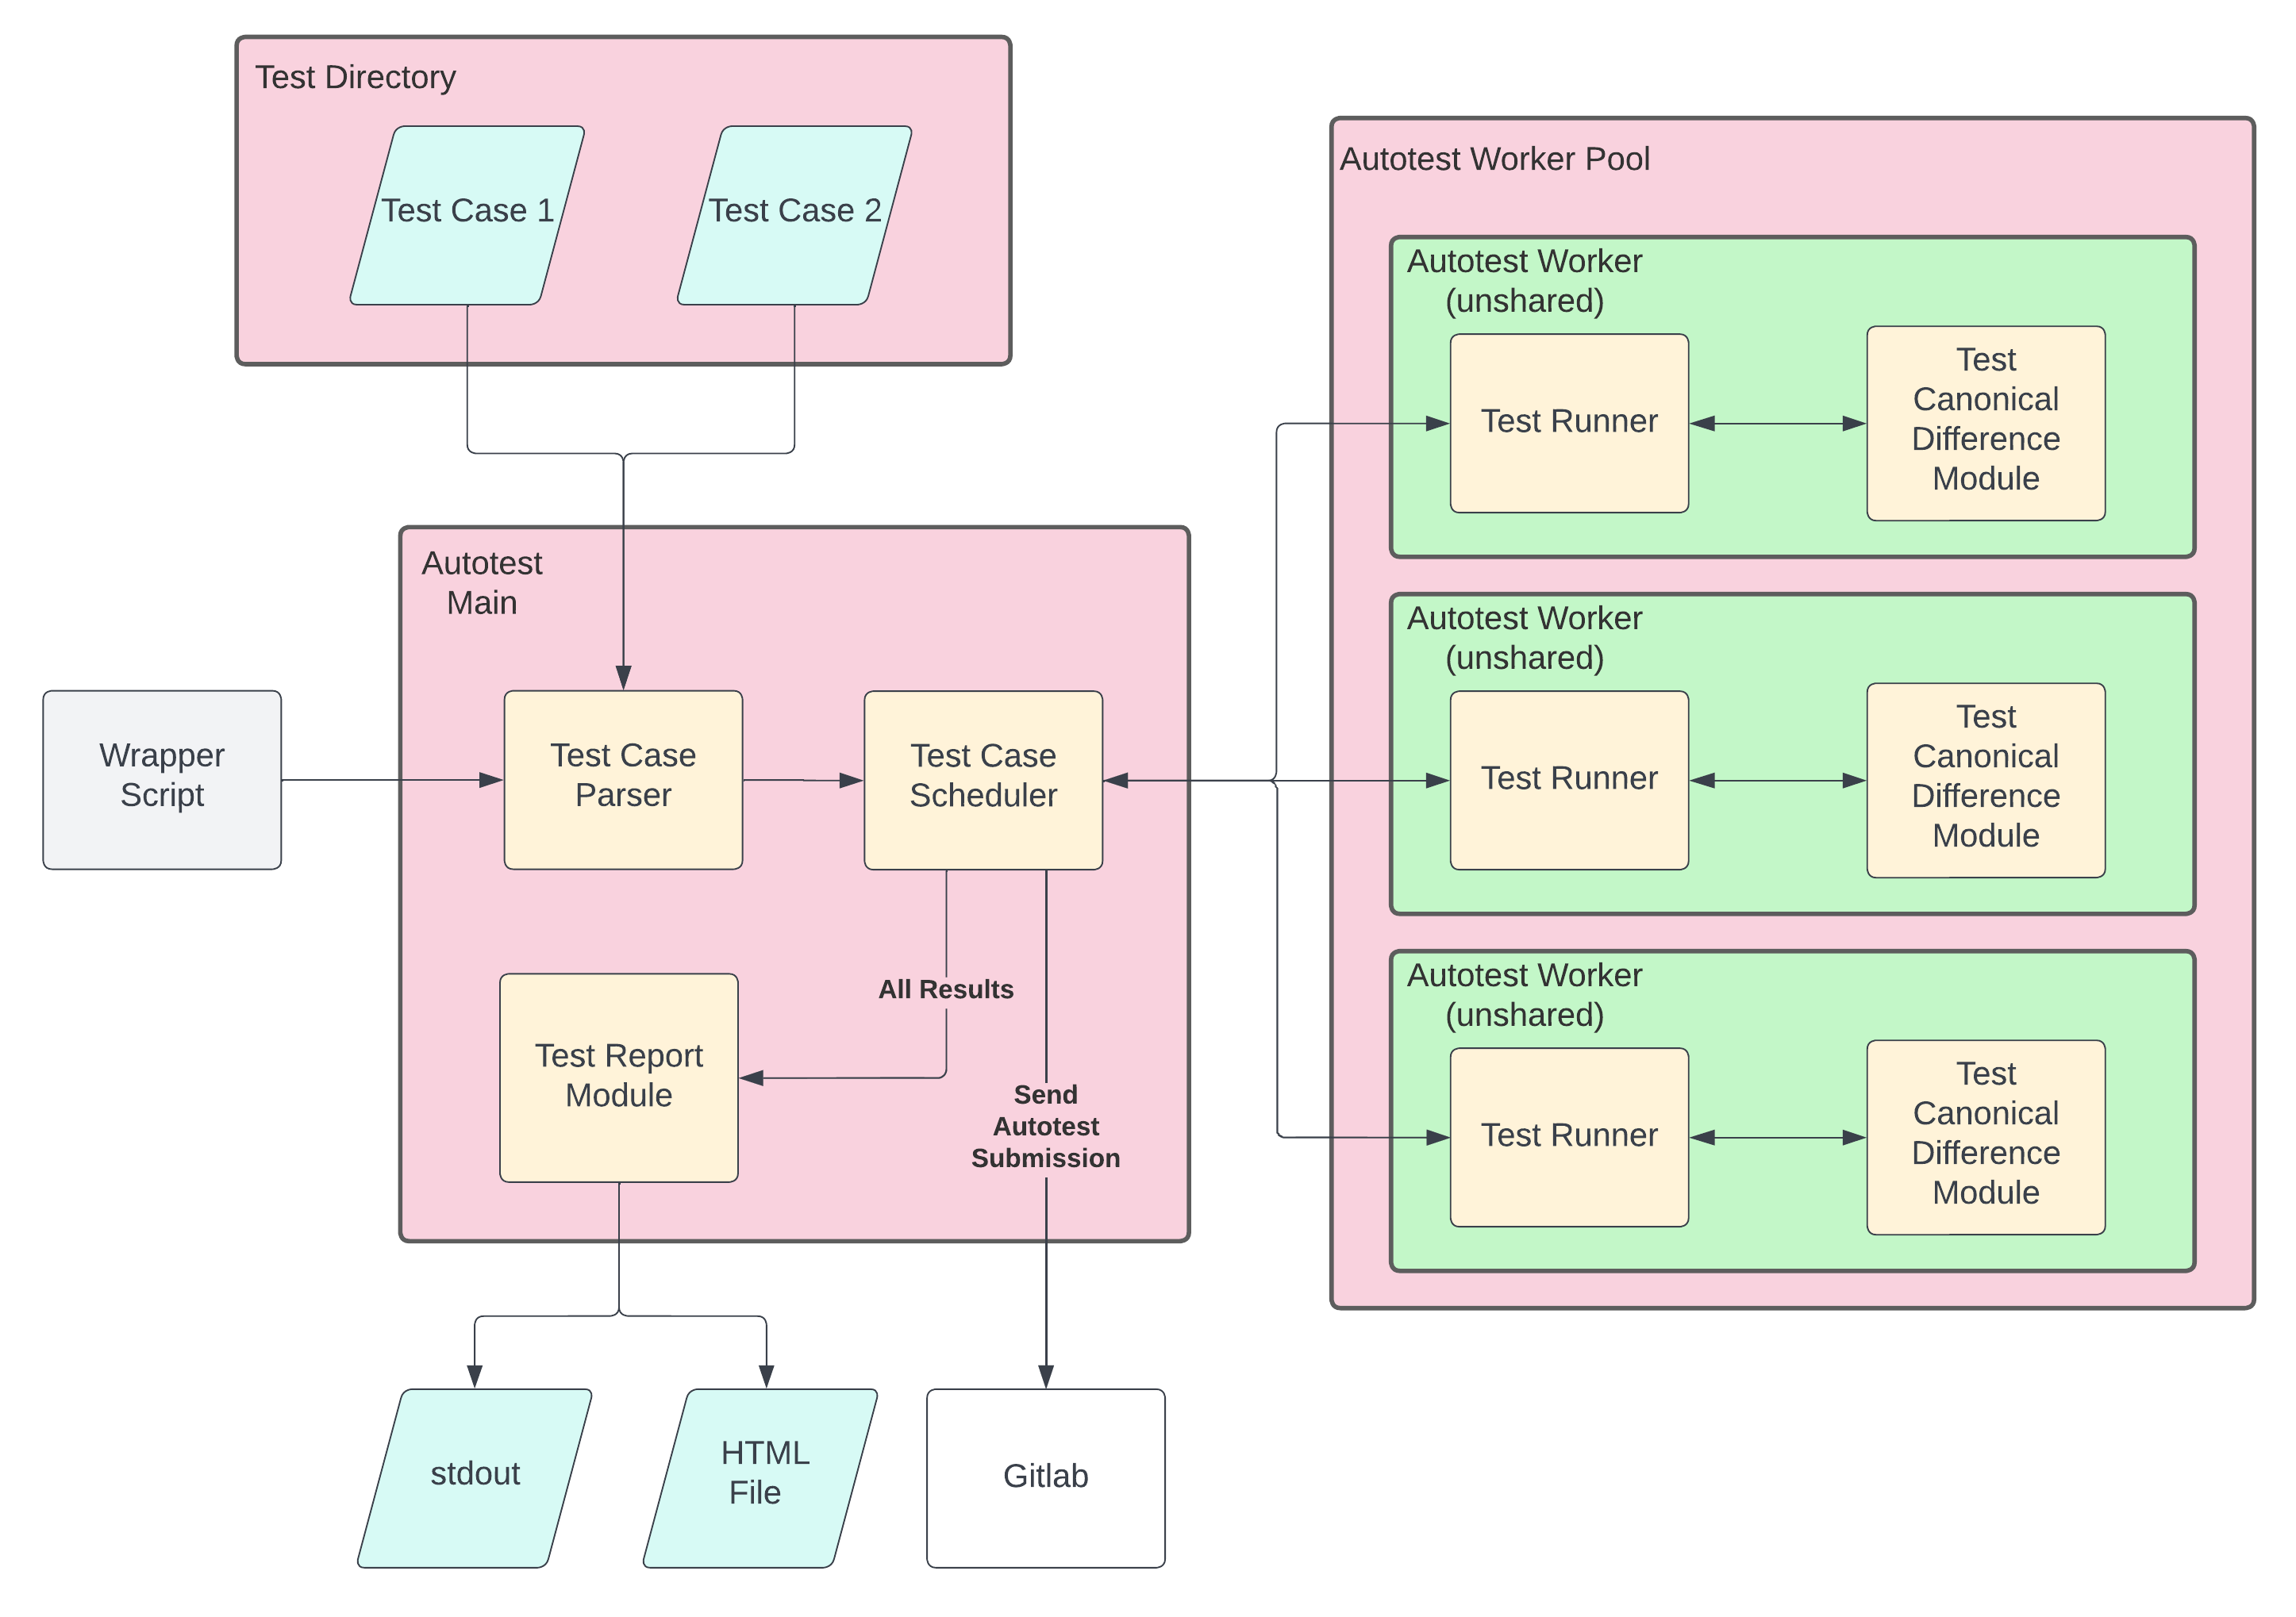
\includegraphics[width=\textwidth, height=0.85\textheight, keepaspectratio=true]{architecture}
	\end{figure}
\end{frame}
\subsection{Modules}
\begin{frame}
	\frametitle{Core Module}
	\textbf{Purpose:} The ``Main" Program\\
	\begin{itemize}
		\item Coordinates execution of modules
			\pause
		\item Facilitates information transfer between modules
			\pause
		\item Exposed only to the abstraction of each module
			\pause
		\item Direct code only for optional ``administrative" tasks
			\begin{itemize}
				\item Upload submission to UNSW GitLab
					\pause
				\item Upload autotest results to UNSW CSE
			\end{itemize}
	\end{itemize}
\end{frame}

\begin{frame}
	\frametitle{Parser Module}
	\textbf{Purpose:} Argument and Test Case Parser\\
	\begin{itemize}
		\item Ingests autotest parameters for processing into usable information
			\pause
		\item Retrieves relevant autotest test cases and processes them into test definitions
			\pause
		\item Minimised exposure to test definition
			\pause
		\item Most complex component in the entire package
			\pause
	\end{itemize}
	\textbf{Changes:}
	\begin{itemize}
		\item Legacy parser code carries too much technical debt for a refactor (circular dependency hell etc.)
			\pause
		\item Writing a new one is unrealistic due to time and correctness concerns
			\pause
	\end{itemize}
	\textbf{Status:} Salvaged/Ported legacy + adaptor
\end{frame}

\begin{frame}
	\frametitle{Test Case Definition}
	\textbf{Purpose:} Defines a test and the information contained within it\\
	\begin{itemize}
		\item Used by the parser to generate the test definitions to be scheduled and executed
			\pause
		\item Contains all information involving each test such as required files, pre-checks, execution instructions etc.
			\pause
		\item Used by the runner to execute the test itself
			\pause
		\item Easily expanded for new features and improvements
			\pause
	\end{itemize}
	\textbf{Status:} Completed - Improvements (further decoupling etc.)
\end{frame}

\begin{frame}
	\frametitle{Test Case Scheduler Module}
	\textbf{Purpose:} Test runner pool manager and test allocator\\
	\begin{itemize}
		\item Utilises given parameters to initialise and setup a container pool that enables concurrent execution of tests
			\pause
		\item Schedules ingested test definitions to free workers in container pool via producer-consumer pattern with synchronisation primitives
			\pause
		\item Manages worker instances and cleanup on completion/process signal
			\pause
		\item Delivers the most performance benefit by enabling parallel execution of tests which decreases testing time when additional CPU threads are available compared to legacy that will only ever utilise one thread
			\pause
	\end{itemize}
	\textbf{Status:} Completed
\end{frame}

\begin{frame}
	\frametitle{Test Case Runner Module}
	\textbf{Purpose:} Container management and test runner\\
	\begin{itemize}
		\item Initialises a worker which accepts test definitions until no more can be found or signal sent
			\pause
		\item Utilises novel pure-python container implementation to enable compartmentalised execution of a given test
			\pause
		\item Manages container environment setup and cleanup for each test
			\pause
		\item Expected to deliver on security needs as containerisation minimises the damage to the host system in the event unintended or malicious actions are performed by a test case
			\pause
	\end{itemize}
	\textbf{Status:} Completed - Improvements (further configuration etc.)
\end{frame}
\begin{frame}
	\frametitle{Why do we need containerisation?}
	\begin{itemize}
		\setlength\itemsep{1em}
		\item Many courses run autotest with their class account (cs1521) when marking which has led to concerns of malicious programs inheriting an overly privileged user id
			\pause
		\item We can fix this by having a \textbf{autotest worker} execute tests in an isolated container to eliminate most risks of damage on the host file system
			\pause
		\item In the event the container is ``escaped", we would like to have containerisation \textbf{\underline{without the need for root access (rootless)}} to limit the damage associated with inheriting root permissions
	\end{itemize}
\end{frame}
\begin{frame}
	\frametitle{Why a novel container implementation?}
	In most cases, writing your own container implementation is a terrible idea
	\pause
	\\~\\
	For this project, a suitable existing container engine could not be found:
	\begin{itemize}
		\setlength\itemsep{1em}
		\item Docker, Bubblewrap etc. have too much overhead and are too powerful for the job
			\pause
		\item Rootless container engines exist but they are considered to be inferior and task-specific support/documentation has been minimal
			\pause
		\item Various pure-python container projects rely on the \textit{setns(2)} system call which requires root permissions
			\pause
	\end{itemize}
	Most of these container engine projects wrap around the \textit{unshare(2)} system call to deliver capabilities
\end{frame}
\begin{frame}
	\frametitle{Novel container details}
	In the interest of time, only an overview of sandbox will be presented\\
	Specific details will be available in the final report
	\begin{itemize}
		\setlength\itemsep{0.75em}
		\item Written entirely in Python and easily used via \textit{with} statement
			\pause
		\item Rootless container engine with no visible alternatives on Github
			\pause
		\item Provides \textit{chroot} functionality with additional isolation provided by namespaces via \textit{unshare(2)}
			\pause
		\item Container file system is mostly isolated from host with configuration options available to expose additional directories as both read-only or read-write
			\pause
		\item Sandbox namespace isolation is irreversible for a specific Python interpreter process due to it's rootless nature as \textit{setns(2)} requires root
	\end{itemize}
\end{frame}

\begin{frame}
	\frametitle{Test Case Canonical Difference Module}
	\textbf{Purpose:} Test correctness checker and test case report generation\\
	\begin{itemize}
		\item Compares output of executed test to expected output
			\pause
		\item Reports success when output matches expected
			\pause
		\item Reports failure when output does not match expected with a report on differences and test reproduction information
			\pause
		\item Should report similar if not better information than what legacy currently provides
			\pause
	\end{itemize}
	\textbf{Status:} Semi-Completed - Coupled with Test Definition but decoupled as much as possible in a semi-modular fashion (isolated into it's own function)
\end{frame}

\begin{frame}
	\frametitle{Test Case Report Module}
	\textbf{Purpose:} Optional HTML report generation\\
	\begin{itemize}
		\item Converts autotest output to more readable HTML form
			\pause
		\item Assists in course administration with forums by making output much more easier to copy by students
			\pause
	\end{itemize}
	\textbf{Status:} Dropped - Easily implemented into the Core module (suitable implementation area already marked)
\end{frame}

\section{Demonstration \& Evaluation}
\subsection{Demonstration}
\begin{frame}
	\frametitle{Demonstration}
	\textbf{Let's see the new autotest (interim name: lemontest) in action on the following compared to legacy:}
	\\~\\
	\begin{itemize}
		\setlength\itemsep{1em}
		\item \textbf{COMP1521 C Exercise:} float\_2048
		\item \textbf{COMP1521 MIPS Exercise:} ackermann
		\item \textbf{COMP1521 MIPS Assignment:} connect\_four (no comparison to legacy as it is not available)
		\item \textbf{Local pytest on standard tests:} Ideally automated but GitHub Actions did not support proper execution of lemontest
	\end{itemize}
\end{frame}
\subsection{Evaluation}
\begin{frame}
	\frametitle{Evaluation - Test Environment}
	\begin{itemize}
		\setlength\itemsep{1em}
		\item The server used for evaluating preliminary results is the UNSW CSE \textit{nw-k17-login1} server with 4 available CPU threads
			\pause
		\item Test cases are identical with only the introduction of lemontest exclusive parameters such as \textit{worker\_count} and other parameters that are necessary for test execution
			\pause
		\item The preliminary evaluation is only in respect to the float\_2048 C exercise with more formalised results to come in the report
			\pause
		\item Performance gains from using lemontest depend on the hardware and the resources available to the executing user (little performance gain expected from parallelisation if only one thread is available)
	\end{itemize}
\end{frame}
\begin{frame}
	\frametitle{Evaluation - Error-free Programs}
	For testing of programs that compile correctly and have no runtime issues for the float\_2048 C exercise (averaged over 10 executions):\\
		\pause
	\begin{itemize}
		\setlength\itemsep{0.75em}
		\item A testing time \textbf{reduction} of \textbf{\underline{58.5\%}} is observed with lemontest over 11 test cases \textbf{(51.305s vs 123.831s)}
			\pause
		\item A testing time \textbf{reduction} of \textbf{\underline{12.8\%}} is observed with lemontest over 1 test case \textbf{(26.034s vs 29.875s)}
			\pause
		\item The less than expected performance gain for both cases when compared to the legacy autotest implementation is attributed to overhead introduced with lemontest via containerisation of tests
			\pause
		\item It is noted from Shrey Somaiya, ``Can we gain performance by disabling containerisation?", a testing time \textbf{increase} of \textbf{\underline{7.1\%}} was observed when disabling containerisation for lemontest \textbf{(54.985s vs 51.305s)}
	\end{itemize}
\end{frame}
\begin{frame}
	\frametitle{Evaluation - Runtime Error Programs}
	For testing of programs that compile correctly but have runtime errors for the float\_2048 C exercise:\\
	\pause
	\begin{itemize}
		\setlength\itemsep{0.75em}
		\item The massive increase in testing time has been attributed to an issue with how DCC compiled binaries work on CSE
			\pause
		\item The issue itself has been identified but it seems to only occur on CSE and was not able to be reproduced locally
			\pause
		\item DCC issues are out of scope for this thesis so a reasonable evaluation on performance could not be performed for programs with runtime errors
	\end{itemize}
\end{frame}

\section{Conclusion}
\subsection{Analysis \& Contributions}
\begin{frame}
	\frametitle{Analysis \& Contributions}
	\begin{itemize}
		\setlength\itemsep{1em}
		\item Transition testing ready implementation of new autotest package
			\pause
		\item User experience for course staff is very similar to legacy autotest with minimal changes required for test cases \textbf{(2-3 lines on average per exercise)}
			\pause
		\item User experience for students is very similar to legacy autotest with slight output differences reflecting the isolated and parallelised execution of each test case
			\pause
		\item Designed for ease of understanding and to support feature extensibility
			\pause
		\item Provides better overall performance in the general use case with additional computing resources
	\end{itemize}
\end{frame}
\begin{frame}
	\frametitle{Analysis \& Contributions - continued}
	\begin{itemize}
		\setlength\itemsep{1em}
		\item Unexpected setbacks led to some less-used features being unimplemented but feature parity has been achieved for most use cases
			\pause
		\item Documentation is more extensive than legacy autotest
		\begin{itemize}
			\setlength\itemsep{0.5em}
			\item Significant commenting of code to assist ease of understanding
				\pause
			\item Additional supporting documentation that will assist new courses to consider integrating autotest to reduce manual marking fatigue and minimise errors
		\end{itemize}
	\end{itemize}
\end{frame}
\subsection{Future}
\begin{frame}
	\frametitle{Near Future: Rest of Thesis C}
	\begin{itemize}
		\setlength\itemsep{1em}
		\item Complete documentation of the new autotest package
			\pause
		\item Clean up code and fix any outstanding known bugs
			\pause
		\item Implement any extension or low-priority features if time permits
			\pause
		\item Write the thesis report, with further evaluation and analysis
	\end{itemize}
\end{frame}
\begin{frame}
	\frametitle{Foreseeable Future: To Complete}
	\begin{itemize}
		\setlength\itemsep{1em}
		\item Feature improvements to containerisation
		\begin{itemize}
			\item cgroups v2 support
				\pause
			\item File mounting (only directories supported at the current time)
				\pause
			\item Customised mount targets for both directories and files
				\pause
			\item Improved containerisation roll-back functionality (currently impossible)
				\pause 
		\end{itemize}
		\item Further decoupling of canonical difference module from the test definition class 
			\pause
		\item Verify fixes and performance results once DCC issue has been fixed in regard to delayed process exit
			\pause
		\item Transition UNSW CSE to the new autotest package for further testing within a course like COMP1521 such that any hidden issues can be identified and rectified as necessary
	\end{itemize}
\end{frame}
\begin{frame}
	\frametitle{Distant Future}
	\begin{itemize}
		\setlength\itemsep{1em}
		\item Overhaul of the legacy test case parser module
			\pause
		\item Overhaul of the subprocess protocol for execution of tests (unlikely to have much improvement) 
			\pause
		\item Autotest platform upgraded to become cloud-based such that autotest is accessible to all students on the internet rather than requiring direct access to CSE servers
			\pause
		\item Propagation of autotest package to other educational institutions (legacy autotest is rumoured to have been shared with Western Sydney University)
	\end{itemize}
\end{frame}
\subsection{Summary}
\begin{frame}
	\frametitle{Summary}
	We have covered:
	\begin{itemize}
		\setlength\itemsep{0.5em}
		\item Andrew Taylor autotest and it's issues
			\pause
		\item The thesis statement
			\pause
		\item Design considerations made for the new autotest
			\pause
		\item Design approach and core architecture for the new autotest
			\pause
		\item Modules that combine to provide functionality for the new autotest
			\pause
		\item Demonstration and preliminary evaluation of the new autotest
			\pause
		\item Analysis and contributions of the new autotest
			\pause
		\item What's left for thesis C and the future
			\pause
	\end{itemize}
	\textit{\textbf{Thank you for attending!} Questions?}
\end{frame}
\end{document}
